\documentclass[a4paper]{article}
\usepackage{geometry}
\usepackage[utf8]{inputenc}
\usepackage[T1]{fontenc}
\usepackage[bookmarks,hidelinks]{hyperref}
\usepackage[french]{babel}
\usepackage{pdflscape}
\usepackage{graphicx}
\usepackage{afterpage}
\usepackage{listings}
\usepackage{lmodern}

\title{Rapport du projet de Technologies Objets}
\author{Maxime Arthaud \and Korantin Auguste \and Martin Carton}
\date{11 juin 2013}

\begin{document}
\maketitle 
\tableofcontents
\listoffigures
\newpage

\section{Introduction}
  Ce projet consiste en la création d'une interface utilisateur permettant de
  gérer une scène 3D et à la réalisation d'un moteur de rendu par lancé de
  rayons.

  Comme expliqué dans le rapport d'analyse, nous avons décidé de nous découper
  le travail, de façon à ce qu'une personne fasse l'interface graphique,
  une autre le parseur de fichier et l'écriture d'images au format PPM, et une
  autre travaille particulièrement sur le cœur du raytracer.

\section{Architecture}
  Le projet est donc constitué de deux programmes distincts:
  \begin{description}
      \item[L'interface graphique] Qui devra permettre de créer simplement des
        fichiers représentant des scènes, à passer à notre raytracer.
      \item[Le raytracer] Qui, à partir d'un fichier représentant une scène,
        devra générer un rendu, dans le format d'image de notre choix.
  \end{description}

  \subsection{Écriture d'images PPM}
    Pour écrire les images PPM, nous avons écrit un plugin Java qui permet
    d'enregistrer ce format auprès de \verb+javax.image.ImageIO+ qui propose une
    interface commune pour enregistrer des images dans différents formats. Ainsi
    notre programme peut générer des images au format PPM, mais aussi par
    exemple en PNG.
    
    Le choix de ce format est déterminé par le troisième paramètre d'appel du
    programme (la valeur pas défaut est png, ce format étant plus commun).

    Ce plugin consiste en deux classes \verb+imageio.PPMImageWriterSpi+ et
    \verb+imageio.PPMImageWriterSpi+. La première permet d'indiquer à Java les
    capacité de notre plugin. La deuxième permet d'écrire une image sur un flux
    de sortie quelconque.

  \subsection{Format de fichier}
    Nous avons décidé de mettre à disposition un format de fichier dans lequel
    on peut décrire une scène afin de pouvoir enregistrer celles-ci, ou de la
    générer automatiquement (ce qui nous a même permis de faire quelques
    vidéos).

    Le format de fichier ressemble à ceci:
    \begin{lstlisting}[caption=Exemple de fichier associé à la figure
    \ref{fig:rendusimple}]
//exemple de scene :
Camera(eye=(0, 0, 0), origin=(-0.5, 0, 1.5), abscissa=(1, 0, 0),  \
ordinate=(0, 1, 0), widthPixel=200, heightPixel=200)
AmbientLights(0.2, 0.2, 0.2)
Light(pos=(5, 0, 0), intensity=(0.5, 0.5, 0.5))
Sphere(center=(0, 5, 20), radius=3.14, k_diffuse=(0.6,0.3,0.6))
Plane(p1=(-1,0,30), p2=(1, 0, 30), p3=(0, 1, 30))
    \end{lstlisting}

    \begin{figure}[h]
      \centering{
        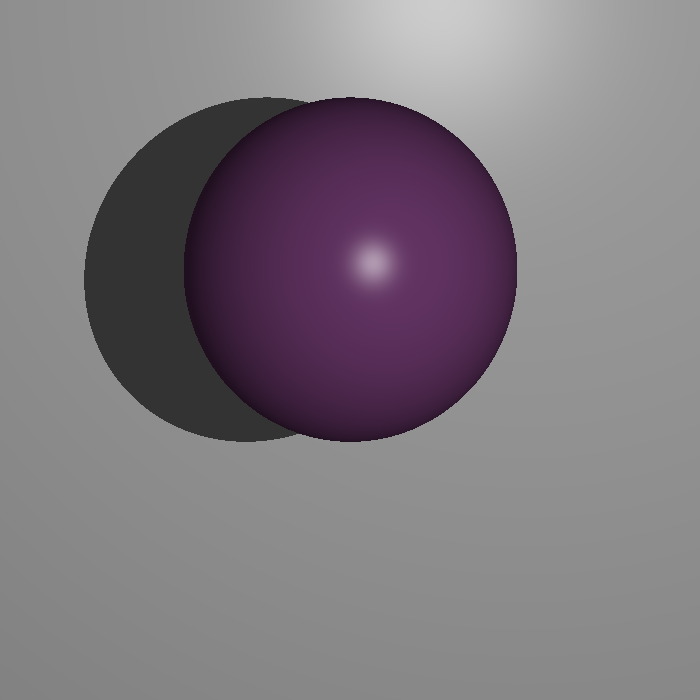
\includegraphics[width=200px]
        {livrables/tests/raytracer/fichier_simple.png}
      }
      \caption{Exemple de rendu simple\label{fig:rendusimple}}
    \end{figure}

    %todo: Korantin veut un fichier casse-sensible
    Il y a un élément par ligne et seule la ligne décrivant au moins une caméra
    est obligatoire. La casse et l'espacement sont ignorés. La plupart des
    propriétés ont une valeur par défaut afin d'éviter de surcharger le
    fichier et de permettre de l'écrire à la main. Des commentaires de fin de
    ligne commençant par «~\verb+//+~» peuvent être insérés.

    Les éléments suivants peuvent être ajoutés:
    \begin{description}
      \item[Camera] décrit une caméra de la scène: elle doit posséder les
        propriétés suivantes:
        \begin{description}
          \item[eye] un point décrivant la position de l'œil;
          \item[origin] un point décrivant l'origine du rectangle de l'écran;
          \item[abscissa et ordinate] les vecteurs qui avec \textit{origin}
            définissent l'écran;
          \item[widthPixel et heightPixem] deux entiers donnant la taille de
            l'image à générer. 
        \end{description}
      \item[AmbientLights] donne les trois composantes primaire de la lumière
        ambiante.
      \item[Light] décrit une source de lumière, elle doit avoir les propriétés
        suivantes:
        \begin{description}
          \item[pos] la position de cette source;
          \item[intensity] l'intensité lumineuse de chaque couleur primaire.
        \end{description}
      \item[Sphere] décrit une sphère, doit avoir les propriétés suivantes:
        \begin{description}
          \item[center] un point représentant le centre de la sphère;
          \item[radius] un flottant représentant le rayon de la sphère.
        \end{description}
      \item[Plane] décrit un plan, doit avoir trois points nommés \textit{P1},
        \textit{P2} et \textit{P3}.
      \item[Triangle] décrit un triangle, doit avoir trois points nommés
        \textit{P1}, \textit{P2} et \textit{P3}.
      \item[Cube] décrit un cube\footnote{En fait les points ne sont pas testés
        pour former un cube, cet objet peut représenter n'importe quel
        parallélépipède.}, doit avoir quatre points nommés
        \textit{P1}, \textit{P2}, \textit{P3} et \textit{P4} répartis comme
        ceci: \begin{lstlisting}
   p2------+
  /|      /|
 / |     / |
p1------p3 |
|  +----|--+
| /     | /
|/      |/
p4------+
        \end{lstlisting}
    \end{description}

    \bigskip
    Les objets \textit{Sphere}, \textit{Plane}, \textit{Triangle} et
    \textit{Cube} peuvent en plus avoir les propriétés suivantes:
    \begin{description}
      \item[brightness] flottant, par défaut à 30. Plus ce nombre est grand, plus la tâche provoquée par la composante spéculaire sera localisée.
      \item[k\_specular] flottant, par défaut à 1. Coefficient par lequel on multiplie la composante spéculaire.
      \item[k\_diffuse] triplet, par défaut à \textit{(1, 1, 1)}. Coefficients
        par lesquels on multiplie les composantes diffuse pour chaque couleur.
        Donne donc la couleur de l'objet.
      \item[k\_reflection] flottant, par défaut à 0. Coefficient par lequel on
        multiplie la composante réfléchie.
      \item[k\_refraction] triplet, par défaut à \textit{(0, 0, 0)}.
        Coefficients par lesquels on multiplie les composantes réfractées pour
        chaque couleur.
      \item[refractive\_index] flottant, par défaut à 1 (la lumière réfractée ne
        sera alors pas déviée). Indice du milieu intérieur à l'objet.
        % todo cela nécessite que l'on parle de l'orientation, notamment pour
        % les TriPoints
    \end{description}

    \bigskip
    Un objet de type \verb+Scene+ est construit à partir d'un tel fichier à
    l'aide la méthode statique \verb+raytracer.FileReader.read+.

  \subsection{Interface graphique}
    Maxime ?

    \begin{figure}[p]
      \centerline{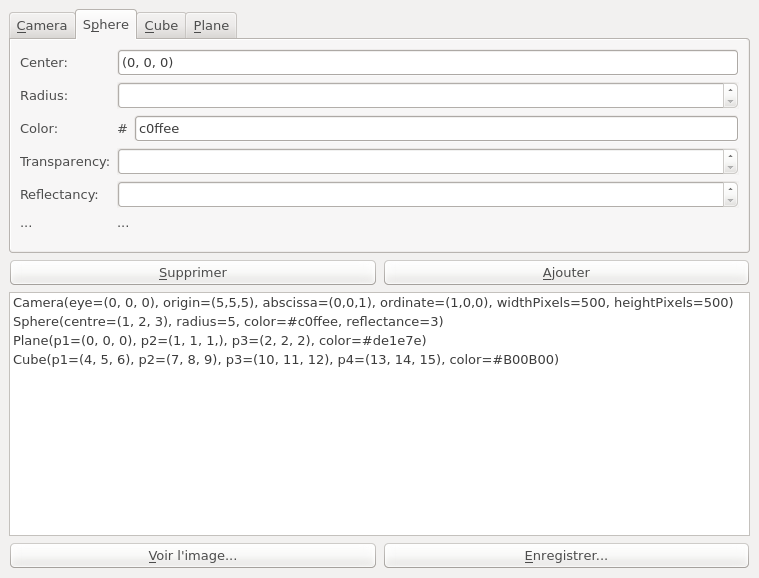
\includegraphics[width=1.2\textwidth]{gui.png}}
    \caption{Interface graphique\label{fig:gui}}
    \end{figure}

    \begin{figure}[p]
      \centerline{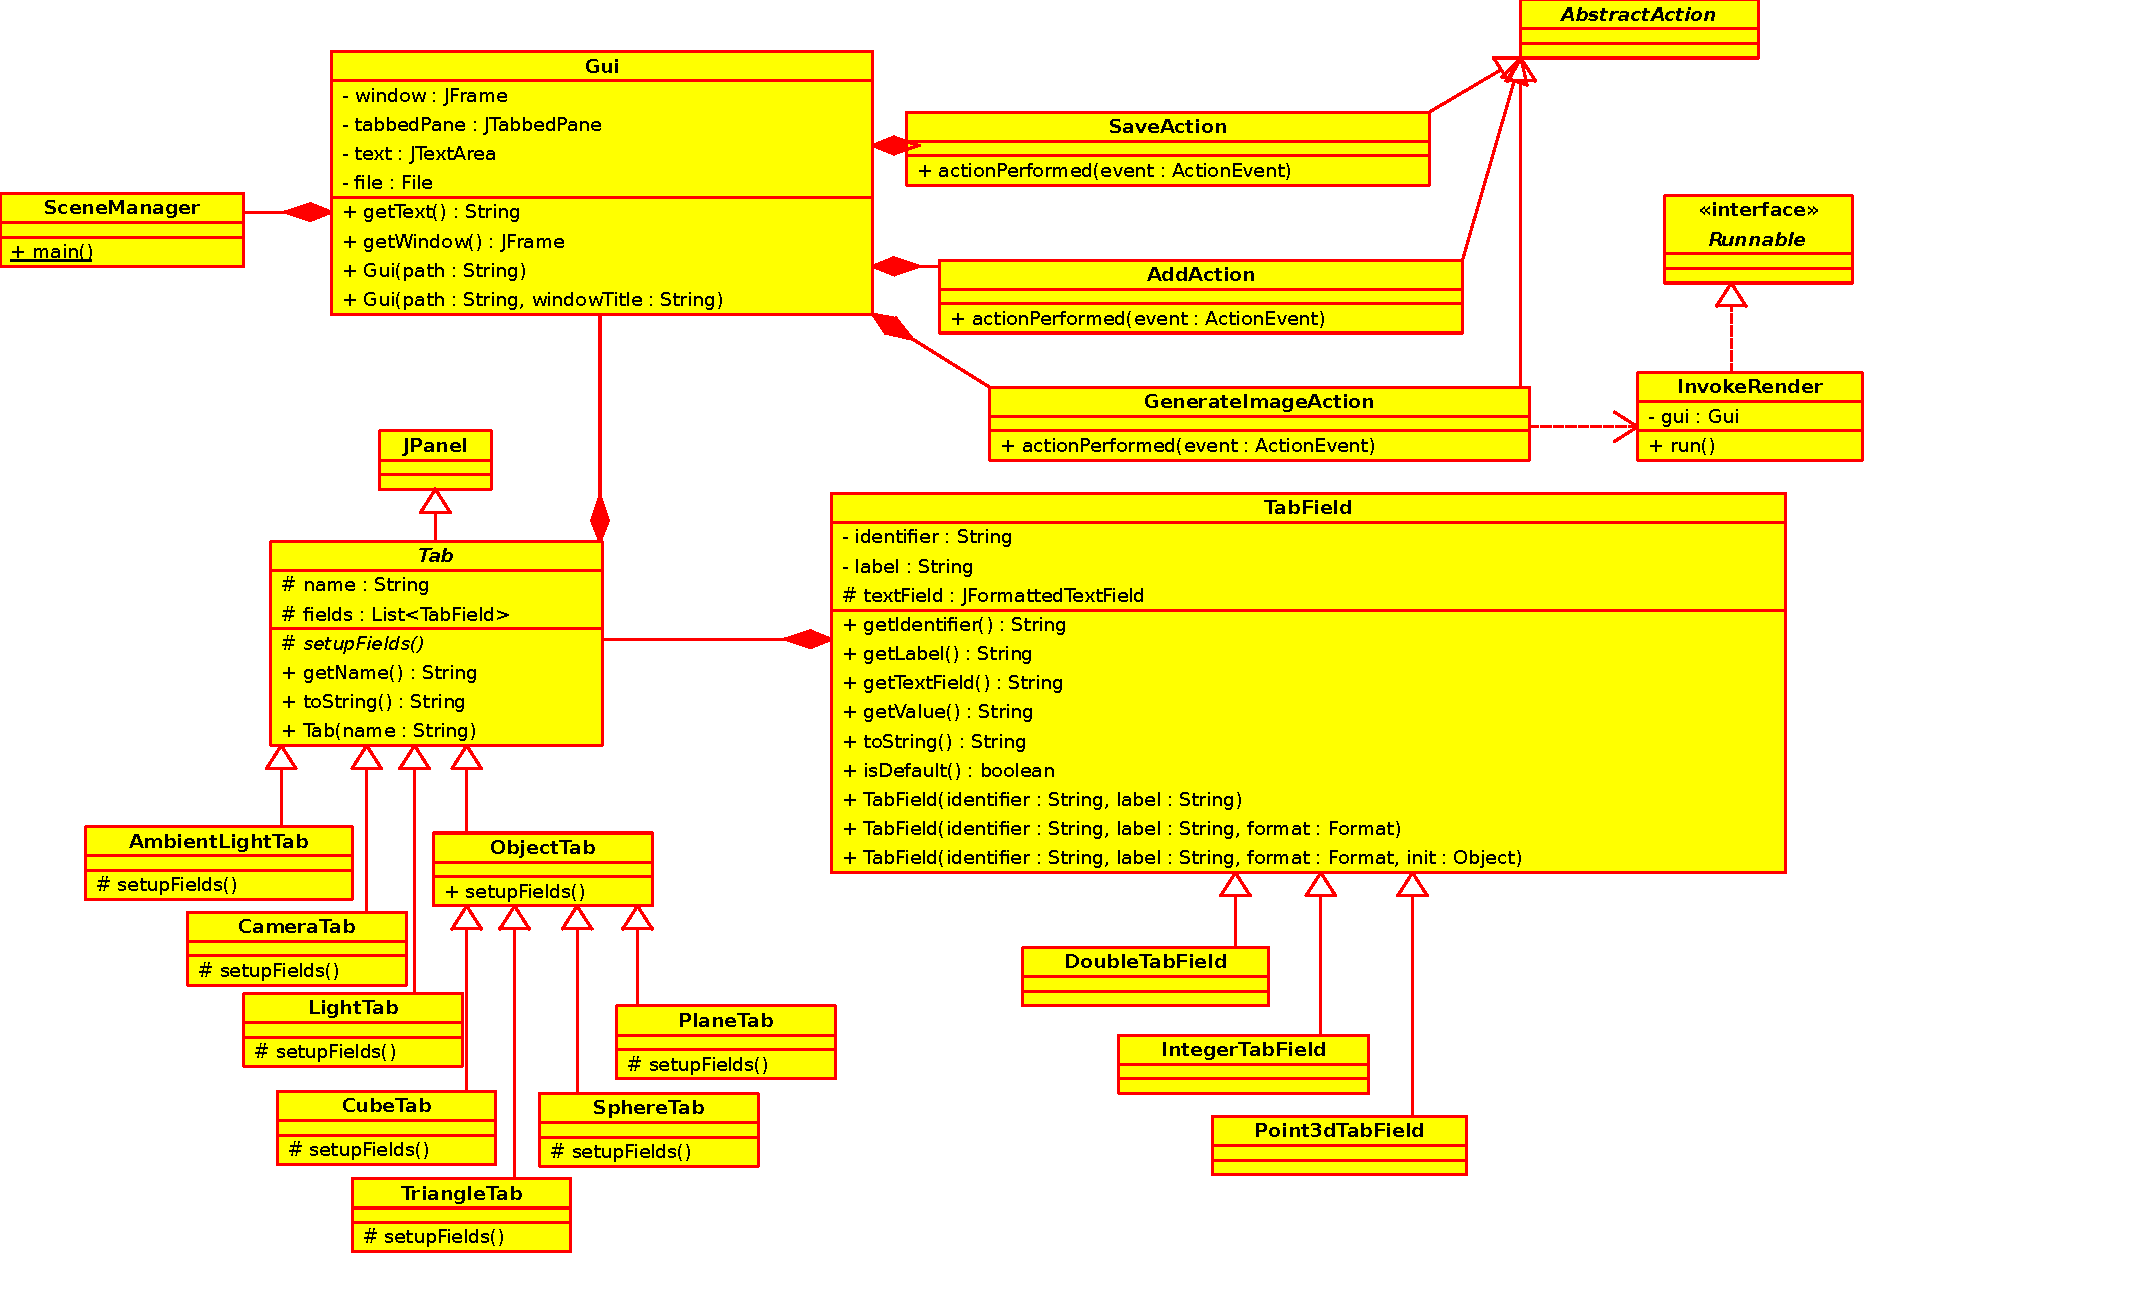
\includegraphics[width=1.2\textwidth]{guiuml.pdf}}
      \caption{Diagramme UML de la GUI\label{fig:guiuml}}
    \end{figure}

  \subsection{Raytracer}
    Pour créer le raytracer, nous avons convenu d'architecturer notre programme
    selon le diagramme de classes suivant présenté en figure \ref{fig:uml}.

    \begin{figure}[p]
      \centerline{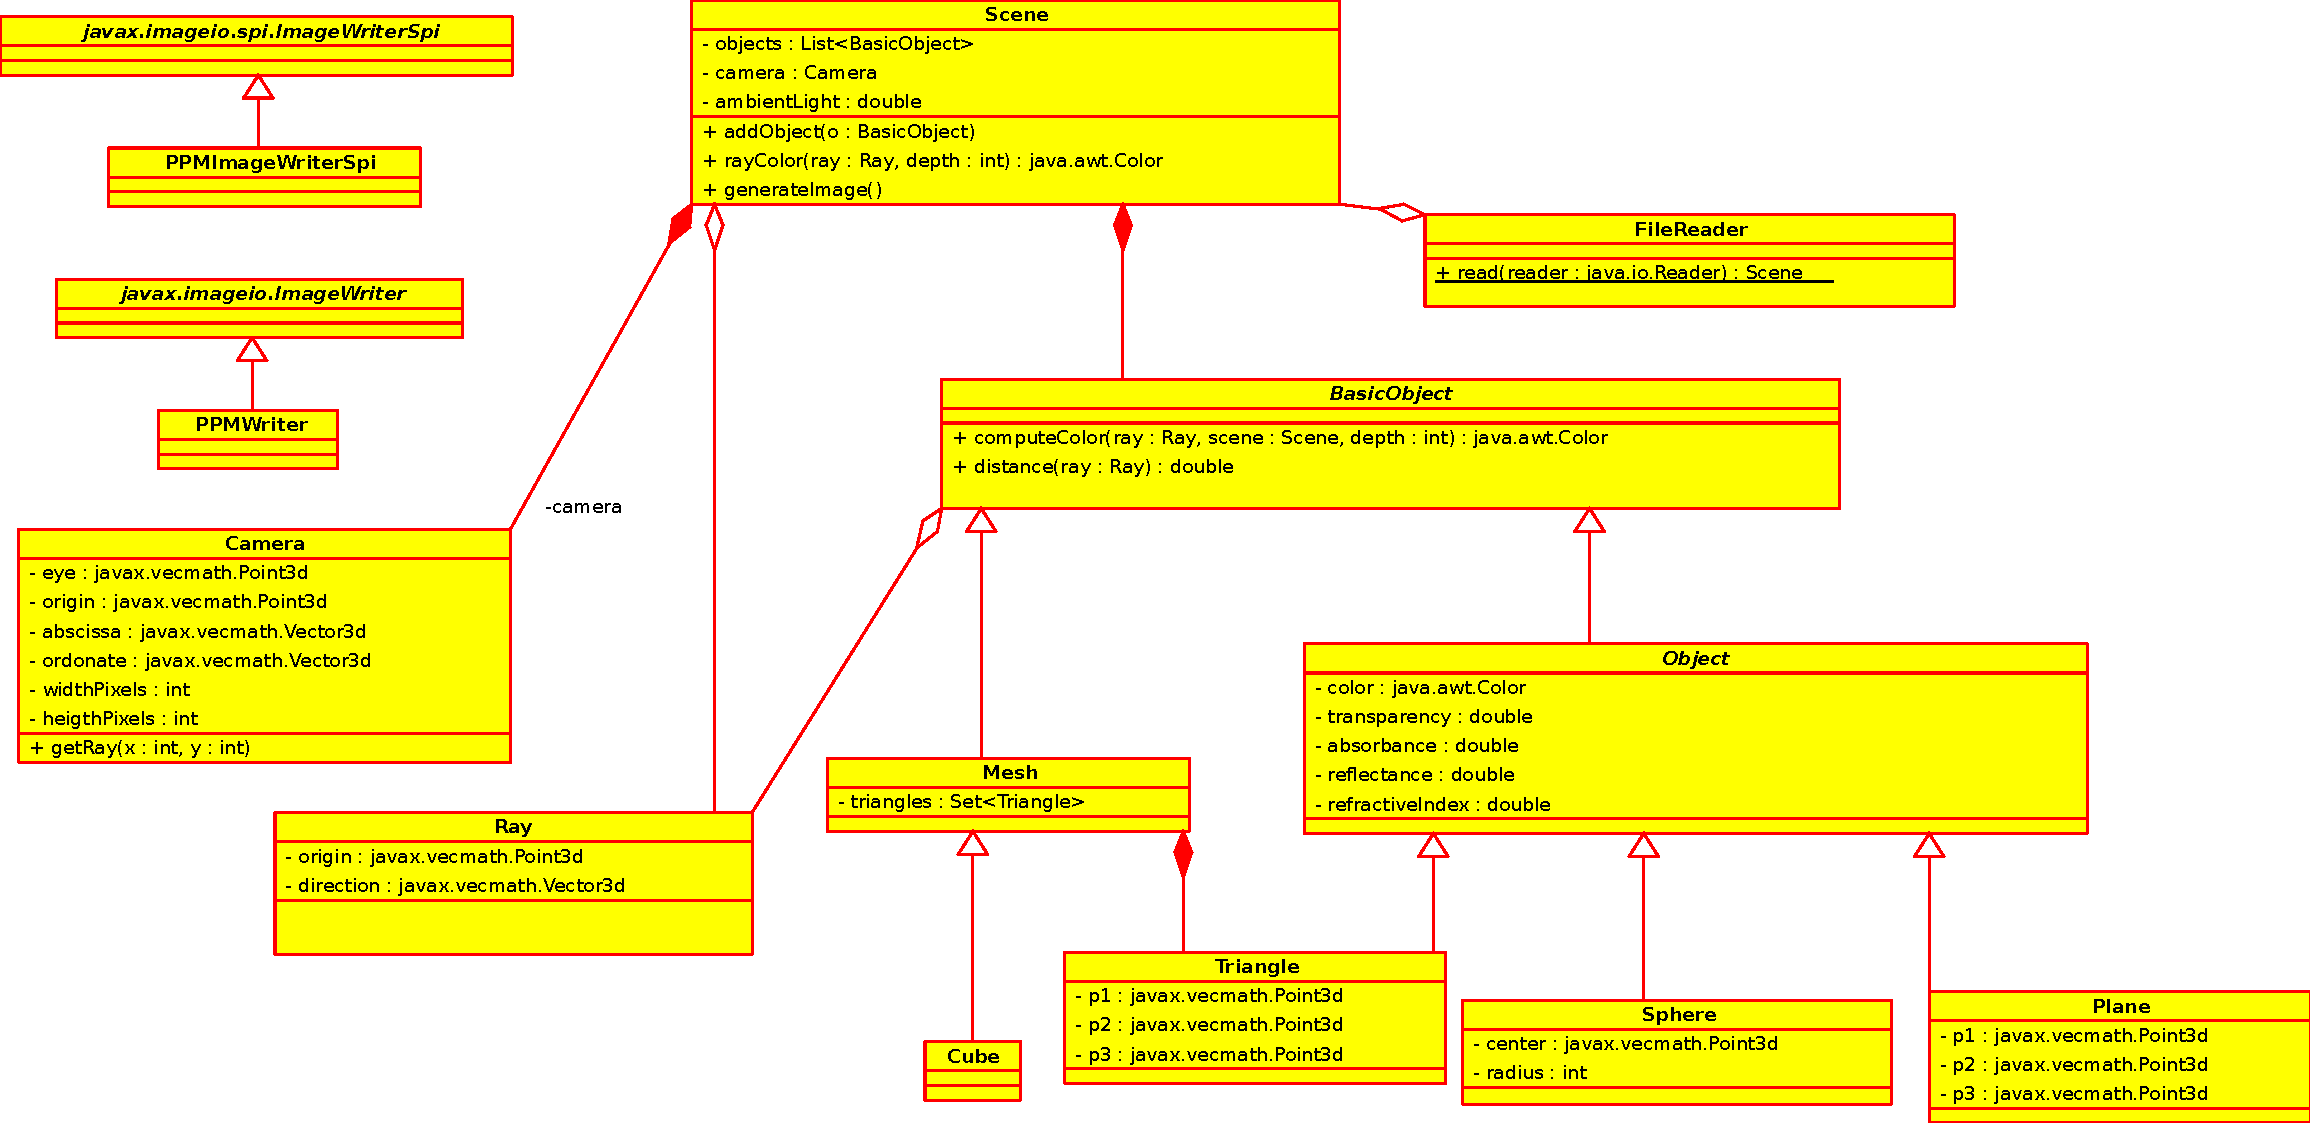
\includegraphics[width=1.2\textwidth]{uml.pdf}}
      \caption{Diagramme UML\label{fig:uml}}
    \end{figure}

    \subsubsection{Changements de conception}
      Par rapport à ce que nous avions prévu lors de notre rapport d'analyse,
      nous avons fait quelques modifications: nous avons rajouté une classe
      pour représenter une lumière, que nous avions oubliée, nous n'utilisons
      pas la classe \verb+java.awt.color+ car il s'est avéré plus pratique de
      manipuler des \verb+double[]+ et nous n'utilisons pas
      \verb+javax.vectmath+, qui n'est pas installé à l'ENSEEIHT, mais nos
      propres classes.

      Ensuite, une scène peut posséder plusieurs caméras, ce qui permet d'avoir
      plusieurs images de la même scène de plusieurs points de vues différents.
      Nous avons ajouté les méthodes dont nous avons eu besoin à la classe
      \verb+Object+. Les classes \verb+Triangle+ et \verb+Plane+ héritent de
      \verb+TriPointed+ car ces objets ont beaucoup de points en commun: ils
      sont représentables par trois points et les formules qu'il y a derrière
      ces classes sont les mêmes; nous en avons profité pour ajouter une classe
      \verb+Parallelogram+ pour les mêmes raisons.
      
      La classe \verb+Mesh+ qui
      devait représenter un objet composé d'un ensemble de facettes
      triangulaires a été changée pour représenter un ensemble d'objets
      basiques, puisque nous n'utilisions rien de spécifique aux triangles la
      restriction n'était pas nécessaire, bien sûr un objet à facettes
      triangulaires peut être représenté par cette classe.
      
      Enfin nous avons ajouté une classe \verb+Texture+ pour alléger notre
      conception.

    \subsubsection{Fonctionnement}
      L'objet \verb+Scene+ dispose d'une méthode pour calculer la couleur
      d'un rayon passé en paramètre.
      Pour le faire, il va regarder quel objet va intersecter avec le rayon en
      premier, et appeler la méthode \verb+computeColor+ de l'objet en question.

      Cette méthode, définie dans la classe \verb+Object+, va faire tous les
      calculs nécessaires pour calculer les différentes composantes. Pour cela,
      elle peut même appeler à nouveau la méthode \verb+rayColor+ de la classe
      scène, sur les rayons réfléchis ou réfractés.
      Dans ces calculs, elle va appeler la méthode \verb+normal+, qui va donner
      la normale au point d'intersection du rayon avec l'objet, méthode qui sera
      définie dans des sous-classes, en fonction de l'objet.

    \begin{figure}[p]
      \centerline{
        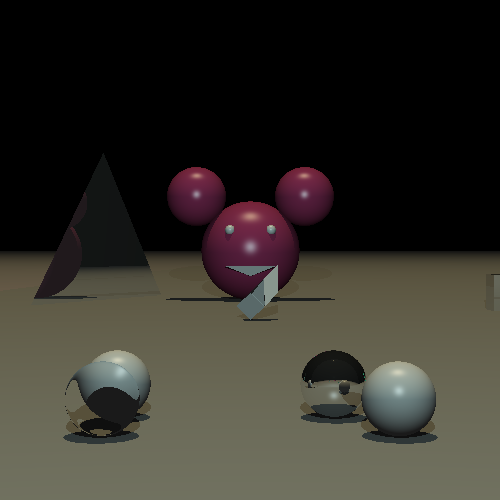
\includegraphics[width=1.2\textwidth]
        {livrables/tests/raytracer/complet.png}
      }
      \caption{Exemple de rendu complexe}
    \end{figure}

    \subsubsection{Problèmes}

    Un problème qui se pose est que, en lançant le rayon avec la méthode \verb+rayColor+ d'une scène,
    à partir d'un point d'intersection avec un objet, l'objet le plus proche qui va intersecter de nouveau
    sera l'objet lui même, à ce même point d'intersection et avec une distance de zéro.
    Pour cela, on aurait pu définir un $\varepsilon$ et vérifier que la distance y soit supérieure, mais
    cela entraînait des problèmes de pixels complètement différent des autres, et il aurait fallu trouver
    une valeur adéquate pour $\varepsilon$. Nous avons donc décidé de ne pas utiliser ce système, et tout
    simplement d'ignorer l'objet qui intersecte, lors du lancer de rayon.
    La méthode \verb+rayColor+ a donc un paramètre (pouvant être nul), qui indique si elle doit ignorer un objet.
    Ce système pose toutefois un problème: un rayon entrant dans une sphère coupera toutefois la sphère en un autre
    endroit. Ce cas est actuellement ignoré, et fait que notre réfraction dans une sphère est peu représentative de la réalité.

    Un autre problème assez important, mais lié à la façon dont le raytracer fonctionne, est qu'un objet transparent ou qui va seulement
    dévier légèrement la lumière, sera capable de masquer les sources lumineuses.
    Cela veut dire qu'il laissera une ombre, alors qu'il est pourtant transparent.

    On peut évaluer la complexité de notre algorithme à du $O(x*y*n*m)$, où:
    \begin{itemize}
        \item $x$ est la largeur de l'image,
        \item $y$ est la hauteur de l'image,
        \item $n$ est le nombre d'objets dans l'image,
        \item $m$ est le nombre de sources lumineuses.
    \end{itemize}

    On voit donc que même si l'algorithme est rapide sur des scènes simples,
    plus la scène contiendra d'objets et de lumières, plus le temps de rendu
    sera élevé, même pour une scène simple, il n'est ainsi pas possible
    d'afficher le rendu en direct dans l'interface graphique.

    \subsubsection{Améliorations}

    % todo Peut-être à virer
    % je vote pour, c'est un peu HS, Martin.
    En changeant la façon dont le raytracer fonctionne, il serait possible d'éviter ce genre de problème: une solution simple est d'utiliser
    des simulations de Monte-Carlo:
    pour obtenir l'éclairement d'un point, on lancera des rayons à partir de ce point, dans des directions choisies au hasard (mais réparties de manière non
    uniforme, pour tenir compte que plus de lumière provient des rayons dans la direction de la normale), et on regardera la lumière diffuse émanera de ces points.
    Ainsi, le problème d'ombre précédemment développé pourra être éliminé.
    Toutefois, cette méthode est très coûteuse en calculs.

    Concernant le temps de rendu sur de grosses scènes, plusieurs choses sont possibles :
    \begin{itemize}
        \item On pourrait paralléliser la génération des images sur tous les
          cœurs disponibles sur l'ordinateur. C'est typiquement quelque chose de
          trivial à paralléliser puisque chaque pixel est généré indépendamment
          des autres (il faudrait cependant modifier nos objets qui conservent
          des données calculés entre les différents appels de méthodes).
        \item Pour chaque source de lumière, plutôt que de parcourir tous les objets pour voir si ils interceptent, on pourrait parcourir seulement qui sont sur le parcours du rayon.
          % todo il manque des mots dans la phrase précédente.
              Pour cela, il nous faudrait diviser notre espace 3D, par exemples à l'aide d'une partition binaire de l'espace (BSP), ou d'un \textit{octree}.
        \item On pourrait aussi profiler le code, et essayer de voir si
          certaines méthodes ne gagneraient pas à être optimisées.
    \end{itemize}

\end{document}

